%%
%% Author: Abby Berkers
%% 14-9-2018
%%
%% Based on contour-plot.tex.

\documentclass{article}  % Standalone class doesn't work.

\usepackage{tikz}
\usepackage{subcaption}  % Subfigures.
\usepackage{fullpage}  % So pictures fit next to each other.

\usetikzlibrary{arrows.meta, decorations.markings}

\begin{document}
    \begin{figure}[h!]
        \centering
        \begin{subfigure}[t]{0.3\textwidth}
            \centering
            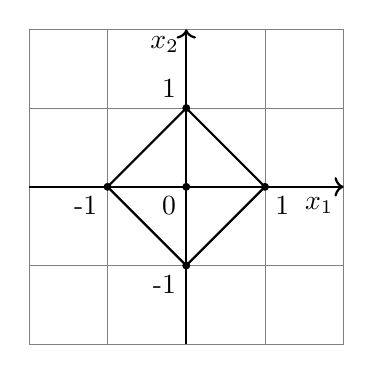
\begin{tikzpicture}[thick]
                \draw[help lines] (-2,-2) grid (2,2);
                % Axes:
                \draw [->] (-2,0) -- (2,0) node [below left]  {$x_1$};
                \draw [->] (0,-2) -- (0,2) node [below left = -1pt] {$x_2$};

                % Axes labels:
                \draw[fill] (-1,0) circle (1pt) node [below left] {-1};
                \draw[fill] (0,-1) circle (1pt) node [below left] {-1};
                \draw[fill] (0,0) circle (1pt) node [below left] {0};
                \draw[fill] (0,1) circle (1pt) node [above left] {1};
                \draw[fill] (1,0) circle (1pt) node [below right] {1};

                % Unit 'circle':
                \draw[rotate = 45] (-0.707, -0.707) rectangle (0.707, 0.707);
            \end{tikzpicture}
            \caption{1-norm}
        \end{subfigure}%
        ~
        \begin{subfigure}[t]{0.3\textwidth}
            \centering
            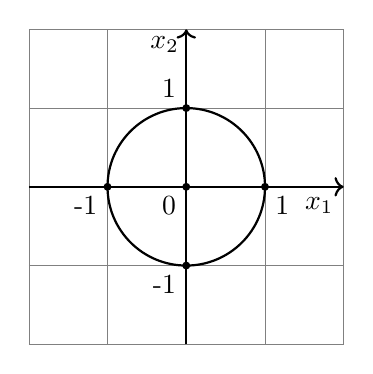
\begin{tikzpicture}[thick]
                \draw[help lines] (-2,-2) grid (2,2);
                % Axes:
                \draw [->] (-2,0) -- (2,0) node [below left]  {$x_1$};
                \draw [->] (0,-2) -- (0,2) node [below left = -1pt] {$x_2$};

                % Axes labels:
                \draw[fill] (-1,0) circle (1pt) node [below left] {-1};
                \draw[fill] (0,-1) circle (1pt) node [below left] {-1};
                \draw[fill] (0,0) circle (1pt) node [below left] {0};
                \draw[fill] (0,1) circle (1pt) node [above left] {1};
                \draw[fill] (1,0) circle (1pt) node [below right] {1};

                % Unit 'circle':
                \draw (0,0) circle [radius = 1];
            \end{tikzpicture}
            \caption{2-norm}
        \end{subfigure}%
        ~
        \begin{subfigure}[t]{0.3\textwidth}
            \centering
            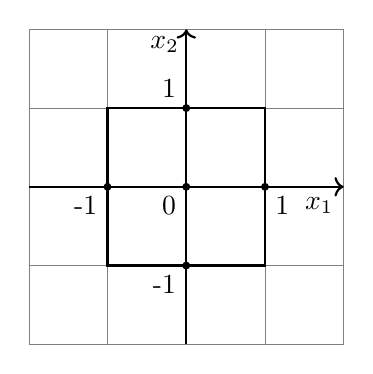
\begin{tikzpicture}[thick]
                \draw[help lines] (-2,-2) grid (2,2);
                % Axes:
                \draw [->] (-2,0) -- (2,0) node [below left]  {$x_1$};
                \draw [->] (0,-2) -- (0,2) node [below left = -1pt] {$x_2$};

                % Axes labels:
                \draw[fill] (-1,0) circle (1pt) node [below left] {-1};
                \draw[fill] (0,-1) circle (1pt) node [below left] {-1};
                \draw[fill] (0,0) circle (1pt) node [below left] {0};
                \draw[fill] (0,1) circle (1pt) node [above left] {1};
                \draw[fill] (1,0) circle (1pt) node [below right] {1};

                % Unit 'circle':
                \draw (-1, -1) rectangle (1, 1);
            \end{tikzpicture}
            \caption{$\infty$-norm}
        \end{subfigure}
        \caption{Unit spheres with respect to different norms.}
        \label{fig:unit-spheres}
    \end{figure}
\end{document}